% This version of CVPR template is provided by Ming-Ming Cheng.
% Please leave an issue if you found a bug:
% https://github.com/MCG-NKU/CVPR_Template.

% \documentclass[review]{cvpr}
\documentclass[final]{cvpr}

\usepackage{times}
\usepackage{epsfig}
\usepackage{graphicx}
\usepackage{amsmath}
\usepackage{amssymb}
\usepackage{multirow}
\usepackage{booktabs}
\usepackage{verbatim}
\usepackage{xcolor}
\usepackage{float}
\usepackage{subcaption}
\usepackage{tabularx}

% footnote
\usepackage[symbol]{footmisc}
\renewcommand{\thefootnote}{\fnsymbol{footnote}}
% \usepackage{titlesec}

\newcommand{\note}[1]{{\bf{\textcolor{red}{note: #1}}}}
\newcommand{\TODO}[1]{{ \textcolor{red}{TODO: #1}}} 
\newcommand{\ljnote}[1]{{\bf{\textcolor{blue}{LJ: #1}}}}
\newcommand{\qiunote}[1]{{\bf{\textcolor{purple}{QIU: #1}}}}
% Include other packages here, before hyperref.

% If you comment hyperref and then uncomment it, you should delete
% egpaper.aux before re-running latex.  (Or just hit 'q' on the first latex
% run, let it finish, and you should be clear).
\usepackage[pagebackref=true,breaklinks=true,colorlinks,bookmarks=false]{hyperref}


\def\cvprPaperID{****} % *** Enter the CVPR Paper ID here
\def\confYear{CVPR 2021}
%\setcounter{page}{4321} % For final version only


\begin{document}

%%%%%%%%% TITLE
% \title{\LaTeX\ Author Guidelines for CVPR Proceedings}
\title{3D Space-Time Correspondence using Normal-assisted Random Walk}

% \author{Changyuan Qiu\\
% Department of EECS, University of Michigan\\
% Institution1 address\\
% {\tt\small peterqiu@umich.edu}
% % For a paper whose authors are all at the same institution,
% % omit the following lines up until the closing ``}''.
% % Additional authors and addresses can be added with ``\and'',
% % just like the second author.
% % To save space, use either the email address or home page, not both
% \and
% Second Author\\
% Institution2\\
% First line of institution2 address\\
% {\tt\small secondauthor@i2.org}
% }

\author{
Linyi Jin \kern15pt Changyuan Qiu \kern15pt Zhuowen Shen \kern15pt Yuliang Zhu \\
%\begin{minipage}{\textwidth}
%   \centering
   University of Michigan\\
	{\tt\small \{jinlinyi,peterqiu,mickshen,yuliangz\}@umich.edu}\\
}

%\end{minipage}
% }

% \author{First Author\\
% Institution1\\
% Institution1 address\\
% {\tt\small firstauthor@i1.org}
% % For a paper whose authors are all at the same institution,
% % omit the following lines up until the closing ``}''.
% % Additional authors and addresses can be added with ``\and'',
% % just like the second author.
% % To save space, use either the email address or home page, not both
% \and
% Second Author\\
% Institution2\\
% First line of institution2 address\\
% {\tt\small secondauthor@i2.org}
% }

\maketitle


%%%%%%%%% ABSTRACT
% \begin{abstract}
%   The ABSTRACT is to be in fully-justified italicized text, at the top
%   of the left-hand column, below the author and affiliation
%   information. Use the word ``Abstract'' as the title, in 12-point
%   Times, boldface type, centered relative to the column, initially
%   capitalized. The abstract is to be in 10-point, single-spaced type.
%   Leave two blank lines after the Abstract, then begin the main text.
%   Look at previous CVPR abstracts to get a feel for style and length.
% \end{abstract}

%%%%%%%%% BODY TEXT
%%%% INTRODUCTION

% \footnote[num]{text}

\section{Introduction}
\label{sec:introduction}

Humans have a remarkable ability to understand dynamic scenes from videos including estimating the 3D structure as well as finding correspondence at different time stamps. For example, when opening a fridge, one can track the door of the fridge and estimate the state and shape of the fridge.
Many prior works~\cite{schonberger2016structure, Luo-VideoDepth-2020, lin2019photometric} infer the 3D structure of a static scene from videos. Other lines of works~\cite{sarlin20superglue,CVPR2019_CycleTime,sarlin20superglue, jabri2020walk} solve the ``what went where" \cite{Wills03} problem of dynamic scenes. However, estimating the 3D structure from videos of {\em dynamic} scenes is still a challenging problem. The classical method Structure from Motion (SfM) is limited to only static scenes~\cite{schonberger2016structure, schwarz1978estimating, ozden2010multibody}. In addition, video datasets with annotations for temporal visual correspondences are scarcely available and hard to create, making supervision a bottleneck for object tracking~\cite{li2019joint, wu2013online}. 



% Many prior works modeled video as a spatio-temporal $XYT$ volume by treating time as another dimension apart from spatial information~\cite{carreira2018quo, Niyogi94analyzinggait, DBLP:conf/cvpr/Zelnik-ManorI01}. However, as the object or the camera could move in arbitrary directions, such method has limits that the physical point depicted at position $(x, y)$ in frame $t$ might not have any relation to what we find at that same $(x, y)$ in frame $t + k$  \cite{feichtenhofer2019slowfast, jabri2020walk}. As a consequence, the notion of \textit{temporal correspondence} — ``what went where" \cite{DBLP:conf/cvpr/WillsAB03} — become crucial for learning about objects in dynamic scenes.

% Recent approaches for self-supervised representation learning are highly effective when pairs of matching views are assumed to be known \cite{DBLP:conf/icml/ChenK0H20, DBLP:conf/cvpr/ChopraHL05, DBLP:journals/pami/DosovitskiyFSRB16, DBLP:conf/cvpr/He0WXG20, DBLP:conf/iclr/HjelmFLGBTB19, DBLP:conf/eccv/TianKI20, DBLP:journals/corr/abs-1807-03748, DBLP:conf/cvpr/WuXYL18, DBLP:conf/cvpr/Zelnik-ManorI01}\ljnote{We need to fix citations, some e.g. [4] looks wrong.}, e.g. constructed via data augmentation, yet data augmentation does not seem promising for creating temporal correspondences. 

% adding 3D information to unsupervised tracking.

In this work, we propose to estimate the 3D structure of dynamic scenes by combining a 3D detection system with a self-supervised visual temporal correspondence learning system.
We reconstruct plane structures from video frames and track the reconstructed planes in dynamic scenes. 
The core methodology of this work is highly inspired by~\cite{jabri2020walk} from Jabri \etal. We incorporate 3D planar surfaces information obtained from PlaneRCNN~\cite{liu2019planercnn} of each frame into the framework of~\cite{jabri2020walk}, which offers important geometric constraint for patch affinity prediction in dynamic scenes. 
%\cite{Chella00understandingdynamic, Ullman85theoptical, 879791}. 

% based on the fact that human visual system can recover the 3D shape of moving objects on the basis of motion information alone \cite{Chella00understandingdynamic, Ullman85theoptical, 879791}. 

% PlaneRCNN (patch ,geometric constraint), provides signals for unsupervised learning, cheat classifier.

%%%% RELATED WORKS
\section{Related Works}
\label{sec:related}

%%  3D from RGBs
% SfM (multi view, static scene) - video frames - correspondence 

% (multi view, static scene)
Structure from Motion is a well-studied field that reconstructs 3D structures based on 2D images. 
However, prior works~\cite{sinha2010multi, dani2011single, whelan2015elasticfusion, tamaazousti2011nonlinear, schonberger2016structure, schwarz1978estimating, ozden2010multibody} are limited to static scenes and cannot handle the occlusions caused by dynamic objects. 
Visual SLAM systems~\cite{whelan2015elasticfusion, raposo2016pi, raposo2013plane} capture consistent room-scale and surface-based maps using RGB-D images or videos. They find point or plane correspondences across frames and use geometry to predict the camera location of each frame and a static 3D pointcloud. Aside from using sensor depthmaps, they also assume certain parts of the environment remain unchanged. Our approach, on the other hand, aims to use RGB frames only and work on dynamic scenes.

% Structure from Motion (SfM) is a well-studied field that reconstruct 3D structures based on 2D image sequences. However, many prior works are limited to static scenarios and cannot handle the occlusion well caused by dynamic objects.  \cite{whelan2015elasticfusion} proposes a visual SLAM system that captures consistent room-scale and surface-based maps using RGB-D cameras. Its locally online optimization nature limits its application to static scenes. \cite{sinha2010multi} proposes a SfM technique using vanishing points to match image pairs, which puts constraints on the structure of the scene. \cite{dani2011single} introduces a reduced order observer model for SfM in the static environment. \cite{tamaazousti2011nonlinear} integrates prior knowledge about the scene into the inference of the camera location. Again, it assumes certain parts of the environment remain unchanged. 

% 3D consistency in video 
Recently, many works use deep learning methods to reconstruct 3D structure from images. There have been works to reconstruct normals~\cite{Eigen15,Wang15}, voxels~\cite{Choy20163d,Girdhar16b}, and depth~\cite{Eigen15,Ranftl2020} from 2D images. However, single view 3D cannot guarantee consistency across video frames and cannot handle dynamic scenes. There are also efforts to estimate consistent depth from video frames using temporal correspondences~\cite{karsch2014depth, patil2020don, wang2019recurrent, zhang2019exploiting} or geometric correspondences~\cite{Luo-VideoDepth-2020}. Our approach differs from these works by estimating planes instead of depth, which is a higher level representation. 

% PlaneRCNN PlaneNet (single view) * no correspondence
Our approach builds most heavily on works aiming to produce a planar reconstruction~\cite{liu2018planenet,yang2018recovering,liu2019planercnn,YuZLZG19,chen2020oasis,jiang2020peek}. In particular, we build on PlaneRCNN~\cite{liu2019planercnn}, which detects planes along with their geometric properties and instance masks from a single RGB image. Despite using surrounding frames to improve the detection quality, it only addresses the detection based on a single frame, and does not touch on the application when the temporal correspondence of the targeted image sequence needs to be learned. 

% SfM is also studied upon video frames. PlaneRCNN \cite{liu2019planercnn} detects planes along with their geometric properties and instance masks with a single RGB input image in the top-down fashion. Despite using surrounding frames to improve the detection quality, it only addresses the detection based on a single frame, and does not touch on the application when the temporal correspondence of the targeted image sequence needs to be learned. PlaneNet \cite{liu2018planenet} proposes a DNN for piece-wise planar depthmap reconstruction
% from a single RGB image and trains on the ScanNet video data. Similarly, it only focuses on geometry, depth and segmentation predictions and does not take advantage of the temporal correspondence in the video.

% Depth (multi view, dynamic scene) * no tracking? Yes; and depth is 2.5D

% Monocular depth estimation is an ill-posed problem which usually requires large amounts of data. However the datasets often have different limitations and biases. \cite{ranftl2020towards} tries to make use of diverse depth estimation data sources to train monocular depth estimation models, even though their annotations are incompatible. They approach the problem in a bottom-up way and design scale and shift invariant losses in the disparity space. To alleviate the dependence on the data, \cite{godard2019digging} applies self-supervised learning to predict the depth map.

\cite{CVPR2019_CycleTime, jabri2020walk} aims to learn useful visual representations for visual correspondence from raw videos without any supervision.
Our work builds on~\cite{jabri2020walk} which enforces strong affinity between image patches by learning embedding vectors to guide a random walk across a palindrome of frames. However, the original work suffers from very strict formulation to prevent the network from finding shortcuts during learning. Our approach adds plane normal aside from the embedding vectors to construct the affinity between nodes of adjacent frames. Our hope is that adding extra constraints can help the system to find robust planar correspondence across frames.

% \cite{jabri2020walk} aims to learn useful visual representations for video data that can improve performance on the downstream tasks. By viewing videos as a graph, they aim to enforce that the edges connecting two nodes (image patches) that have strong affinity have larger weights. They formulate the task as maximizing the probability of returning to the initial node in a random work on a graph that is constructed by a palindrome of frames. The probability of walking between two nodes is denoted as the softmax of the product of the affinity matrix between them. The local affinity map provides the possibility of detecting planes in the scene.

% In this work, we aim to compare the two approaches (top-down and bottom-up) to addressing the plane detection problem, while taking advantage of the feature map used for the random walk mentioned in \cite{jabri2020walk}. Unlike \cite{liu2019planercnn}, the temporal correspondence needs to be learned.

\vspace{-0.1in}
% %%%% METHOD
\section{Method}
\label{sec:method}
% $$L_{cyc}^k=L_{CE}(A_t^{t+k}A_{t+k}^t, I)$$
\subsection{Normal-assisted Random Walk}

% \begin{figure*}
%     \centering
%     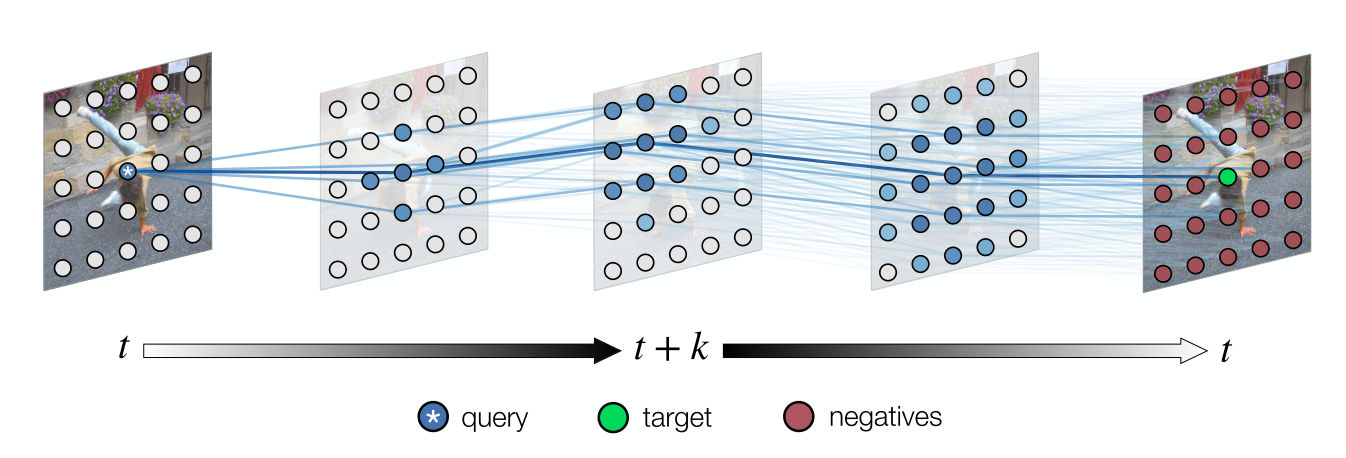
\includegraphics[width=1.0\linewidth]{FinalReport/random_walk.png}
%     \caption{Figure credit \cite{jabri2020walk}. Following there approach, we represent video as a graph, where nodes are image patches, and edges are product of 2D affinities (in some feature space) and 3D distance of detected normal vectors between nodes of neighboring frames.  Our aim is to learn features such that temporal correspondences are represented by strong edges we learn to find paths through the graph by performing a random walk between query and target nodes.  A contrastive loss with affinities times the  encourages paths that reach the target, implicitly supervising latent correspondence along the path. Learning proceeds without labels by training on a palindrome sequence, walking from frame t to t+k, then back to t, using the initial node itself as the target}
%     \label{fig:random_walk}
% \end{figure*}
\begin{figure*}
    \centering
    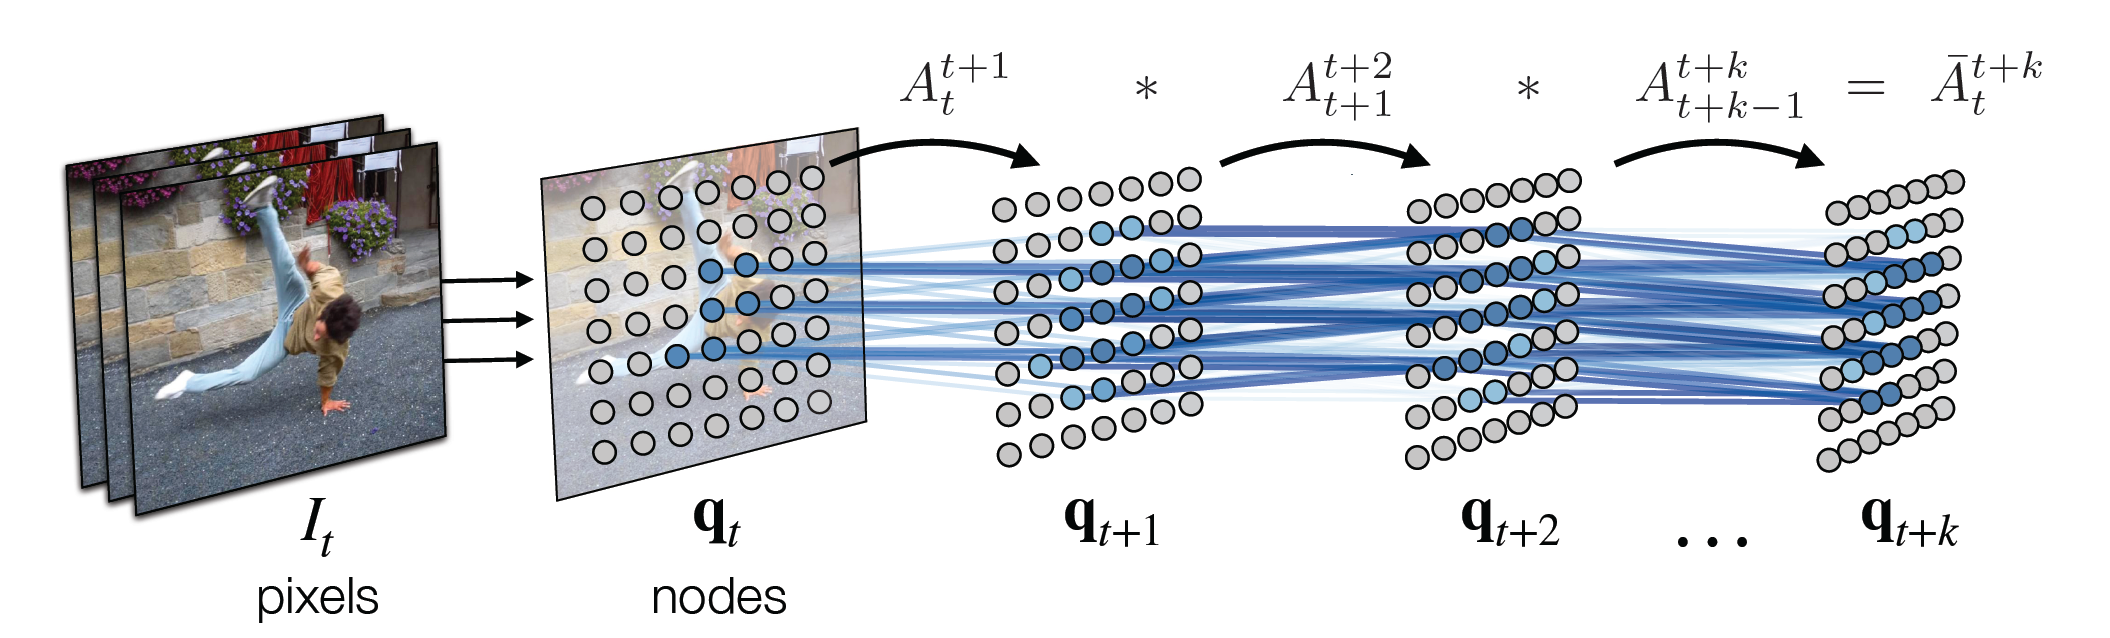
\includegraphics[width=0.8\linewidth]{FinalReport/markov.png}
    \vspace{-0.1in}
    \caption{Figure credit \cite{jabri2020walk}. \textbf{Correspondence as a Random Walk.} We build a space-time graph by extracting nodes from each frame and allowing directed edges between nodes in neighboring frames. The transition probabilities of a random walk along this graph are determined by the product of 2D pairwise similarity in a learned representation and 3D distance of normal vectors detected by a PlaneRCNN network.
    }
    \vspace{-0.1in}
    \label{fig:markov}
\end{figure*}
 \begin{figure*}
    \centering
    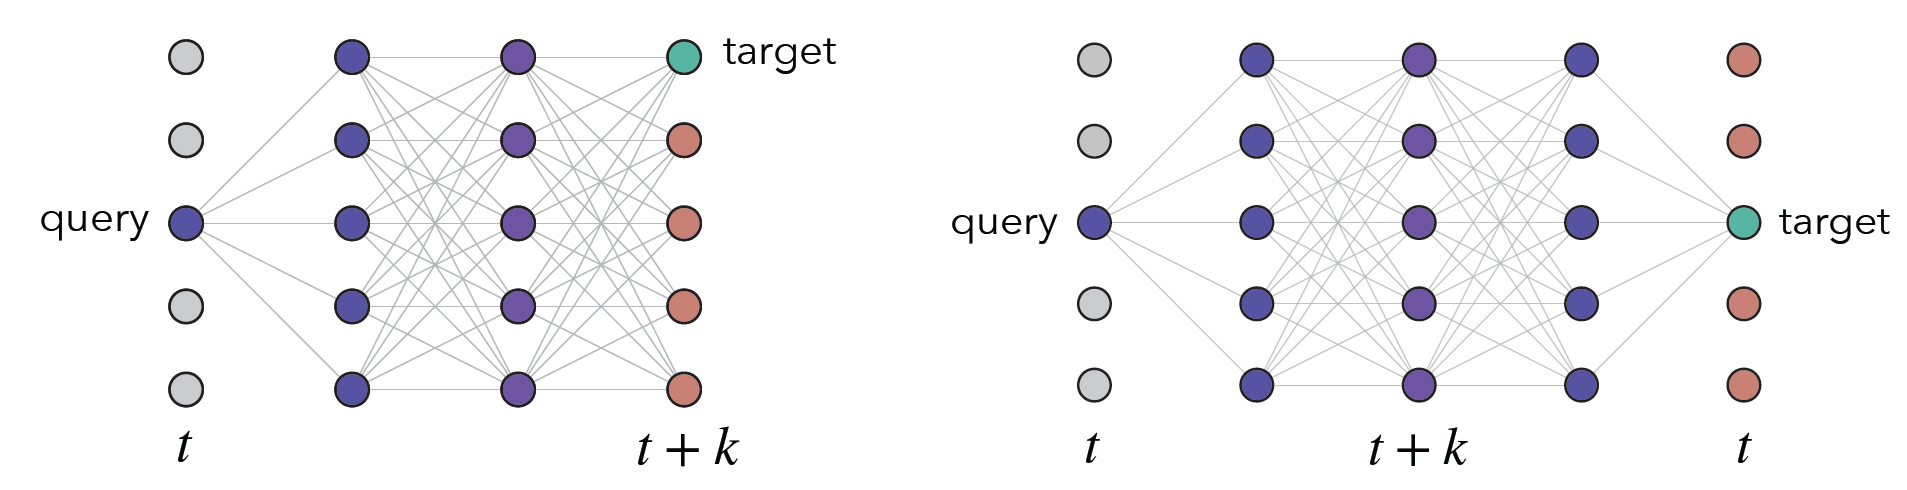
\includegraphics[width=0.8\linewidth]{FinalReport/palindrome.png}
    \vspace{-0.1in}
    \caption{Figure credit \cite{jabri2020walk}. \textbf{Guiding the walk with palindrome self-supervision.} (a) Specifying a target multiple steps in the future provides implicit supervision for latent correspondences along each path (\textit{left}). (b) We can construct targets for free by choosing palindromes as sequences for learning (\textit{right}).
    }
        \vspace{-0.15in}
    \label{fig:palindrome}
\end{figure*}
\vspace{-0.1in}
Following~\cite{jabri2020walk}, we represent each video as a directed graphs with nodes being patches of each frame and edges connect nodes in neighboring frames. Let $\mathbf{I}$ be a set of frames from a video and $\mathbf{q}_{t}$ be the set of $N$ nodes extract from frame $I_{t}$. We train an encoder $\phi$ which maps nodes to $l_2$-normalized $d-$dimensional vectors, which we use to compute a pairwise 2D similarity function between nodes $d_{\phi}(q_{1}, q_{2}) = \langle \phi(q_{1}),\phi(q_{2}) \rangle$ and an 2D embedding matrix for $\mathbf{q}_{t}$ denoted $Q_{t} \in \mathbb{R}^{N\times d}$. We convert pairwise similarities into non-negative affinities by applying a softmax (with temperature $\tau = 0.07$) over edges departing from each node. For timesteps $t$ and $t+1$, the stochastic matrix of 2D affinities is 
\vspace{-0.1in}
\begin{equation}
\small
    A_t^{t+1}(i,j) = \texttt{softmax}(Q_{t},Q^{\text{T}}_{t+1})_{ij} = \frac{\exp(d_{\phi}(\mathbf{q}_{t}^{i}, \mathbf{q}_{t+1}^{j})/\tau)}{\sum_{l=1}^{N}d_{\phi}(\mathbf{q}_{t}^{i}, \mathbf{q}_{t+1}^{l})/\tau)}
\end{equation}



Our modification applies here that we add 3D normal vector distance (normal vector prediction process are detailed in Section \ref{normal}) aside from the 2D embedding affinities to the stochastic matrix.  Let $\mathbf{n}_{t}$ be the set of $N$ normal vector extracted from frame $\mathbf{I}_{t}$, we construct our modified stochastic matrix by multiplying the raw 2D affinity probability $A_t^{t+1}(i,j)$ with the 3D normal eculidean distance $||\mathbf{n}_{t}^{i}-\mathbf{n}_{t+1}^{j}||^2$, and we further apply a softmax to obtain a probability. For timesteps $t$ and $t+1$, our modified stochastic matrix is

\vspace{-0.15in}

\begin{equation}\small
    A_t^{t+1}'(i,j) =  \frac{\exp(A_t^{t+1}(i,j)\cdot ||\mathbf{n}_{t}^{i}-\mathbf{n}_{t+1}^{j}||^2)}{\sum_{l=1}^{N}\exp(A_t^{t+1}(i,j)\cdot ||\mathbf{n}_{t}^{i}-\mathbf{n}_{t+1}^{l}||^2)}
\end{equation}

Note that this describes only the local affinity between the patches of two video frames, $\mathbf{q}_{t}$ and $\mathbf{q}_{t+1}$, and we relate all nodes in the video as a Markov chain following~\cite{jabri2020walk}. Given the spatio-temporal connectivity of the graph, a step of a random walker on this graph can be viewed as performing tracking by \textit{contrasting} similarity of neighboring nodes. Let $X_{t} $ be the state of the walker at time $t$, with transition probabilities $A_t^{t+1}'(i,j) = P(X_{t+1}=j | X_{t} = i)$, where $P(X_t =i)$ is the probability of being at node $i$ at time $t$. And we can formulate long-range correspondence as walking multiple steps along the graph (Figure \ref{fig:markov}):
\vspace{-0.1in}
\begin{equation}\small
A^{t+k}_{t} = P(X_{t+k}|X_{t}) = \prod^{k-1}_{i=0}A_{t+i}^{t+i+1}
\end{equation}
\vspace{-0.1in}
 
 \par \noindent {\bf Guiding the walk with palindrome self-supervision.}
 Our aim is to train the encoder $\phi$ to encourage the random walker to follow paths of corresponding patches as it steps through time. Following~\cite{jabri2020walk}, we train our model with a cross-entrophy loss on the \textit{palindrome} self-supervised training examples. To formalize, given a sequence of frames ($I_t, \dots, I_{t+k}$), we form training examples by simply concatenating the sequence with a temporally reversed version of itself: ($I_t, \dots, I_{t+k}, \dots, I_{t}$). Treating each query node's position as its own target (as shown in Figure \ref{fig:palindrome}), we obtain the following cycle-consistency cross-entropy objective which maximize the likelihood that a walker beginning at a query node at $t$ ends at the same target node at time $t + 2k$:
 \vspace{-0.1in}
\begin{equation}\small
 \mathcal{L}
^{k}_{cyc} = \mathcal{L}_{CE}(A^{t+k}_{t}A^{t}_{t+k}, I) = - \sum_{i=1}^{N} \log P(X_{t+2k}=i|X_{t} = i)
\end{equation}
 
As the model computes a soft attention distribution at every time step, we can backpropagate loss across – and thus learn from – the many alternate paths of similarity that link query and target nodes.
 
\par \noindent {\bf Pixel to nodes.\label{pix}}
We sample $64 \times 64$ patches on a $640\times 480$ image with stride of $32$ to allow overlapping. Following \cite{jabri2020walk} and \cite{long2015fully}, we reuse the convolutional feature map between patches obtained from training for testing instead of processing the patches independently and thus features could be extracted with only a single feed-forward pass.

 \par \noindent {\bf Encoder $\phi$. \label{encoder}}
We use ResNet-18 \cite{he2016deep} for the encoder which outputs a 128-dimensional vector for each patch. We apply a linear projection and $l_2$ normalization after the last average pooling layer and modifies the last 2 \texttt{res3} and \texttt{res4} layer to have stride of 1 instead of 2 following \cite{jabri2020walk}.

% \begin{equation}
%     A_t^{t+1}(i,j) \leftarrow P(X_{t+1}=j|X_t=i)\times||n_i-n_j||^2    
%     \label{eqn:normal-assist}
% \end{equation}


\subsection{Normal Prediction for Patches \label{normal}}
\par \noindent {\bf Plane detection.} We follow PlaneRCNN~\cite{liu2019planercnn} to detect planes in each frame. Instead of using the whole pipeline for prediction, we only use the plane detection network in~\cite{liu2019planercnn} and ignore the segmentation refinement network and warping loss module for simplicity. 
The plane detection network uses ResNet50-FPN~\cite{lin2017feature} as the backbone.
A region proposal network is used to extract box proposals. The plane masks and normals are inferred from features from RoIAlign~\cite{he2017mask}. The PlaneRCNN is supervised by ground truth label on ScanNet generated by fitting planes on the original house mesh provided by~\cite{liu2018planenet}. 
\par \noindent {\bf Patch normal assignment.} For each patch, we calculate the GIoU \cite{Rezatofighi_2018_CVPR} between that patch and each bounding box of the plane masks and assign the normal vector of the mask with the highest GIoU. % GIoU is calculated using the following algorithm:



\subsection{Training Details}
Our Normal-assisted Random Walk network is trained on the Scannet training set, using one Tesla V100 GPU on Colab with learning rate 0.0001, batch size 4 and Adam optimizer with default parameters. The model is trained for 25 epochs. 

Our PlaneRCNN network is implemented in Detectron2 and is trained on the Scannet training set, using 2 GPUs with learning rate 0.001, batch size 16, and SGD optimizer with momentum 0.9. The model is trained for 80k iterations.


\vspace{-0.1in}
%%%% EVALUATION
\section{Experiments}
\label{sec:experiments}
\begin{table*}[t]
\centering
\begin{tabular}{p{0.15\linewidth}p{0.13\linewidth}p{0.13\linewidth}p{0.08\linewidth}p{0.08\linewidth}p{0.08\linewidth}p{0.08\linewidth}p{0.06\linewidth}}
\hline
Method & Resolution & Train Data & $J\&F_m$ & $J_m$ & $J_r$ & $F_m$ & $F_r$\\
\hline
Pretrained \cite{jabri2020walk} & 256 $\times$ 256 &  Kinetics & 72.74 & 73.92 & 74.76 & 71.56 & 69.56\\
\textbf{Ours} w/o normal & 640$\times$480 & ScanNet & 73.08 & 74.34 & \textbf{74.87} & 71.83 & 70.07 \\
\textbf{Ours} w/ normal & 640$\times$480 & ScanNet & \textbf{73.14} & \textbf{74.35} & 74.81 & \textbf{71.93} & \textbf{70.17} \\
\hline
\end{tabular}
 \vspace{-0.1in}
\caption{Video object segmentation results on ScanNet}
 \vspace{-0.15in}
\label{table:quan}
\end{table*}

% \vspace{+0.5in}



% \TODO{What is the data that you are using? What are the hyperparameters? How is the model evaluated? What are the baseline approaches that you are comparing your method with? How does the performance of your method compare with these baseline methods? Tables and figures are efficient ways to convey your experiment results.}
\subsection{Dataset}
\begin{figure*}[!t]
    \centering
    \resizebox{1.0\textwidth}{!}{
    \begin{tabular}{ccccccccc}
    \toprule
    w/o normal
    &\frame{\includegraphics[width=0.15\textwidth]{example_wall/e01_no_normal/0_0_blend.jpg}} 
    &\frame{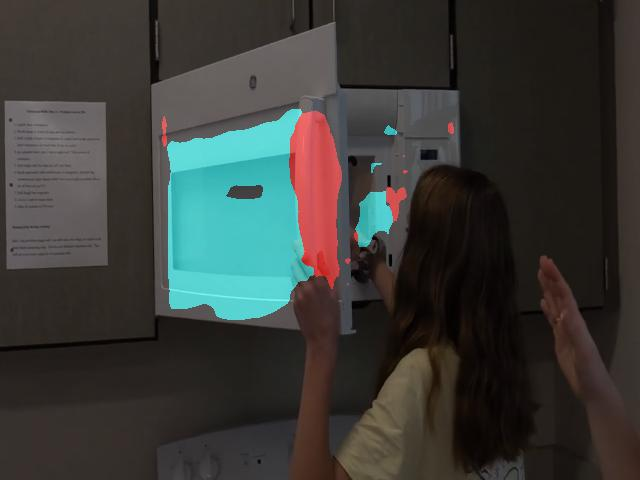
\includegraphics[width=0.15\textwidth]{example_wall/e01_no_normal/0_1_blend.jpg}}
    &\frame{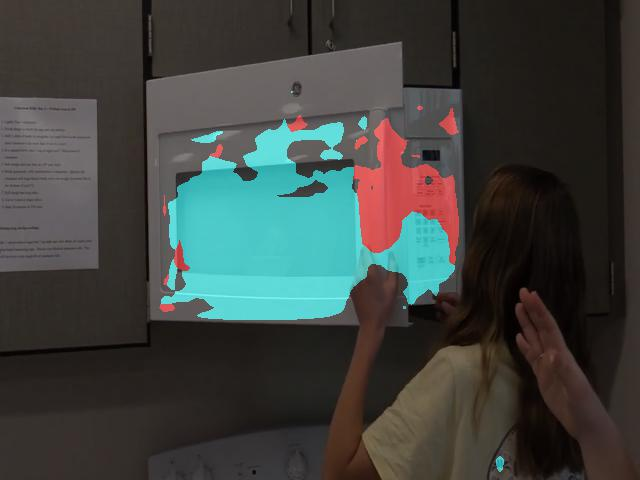
\includegraphics[width=0.15\textwidth]{example_wall/e01_no_normal/0_2_blend.jpg}} 
    &\frame{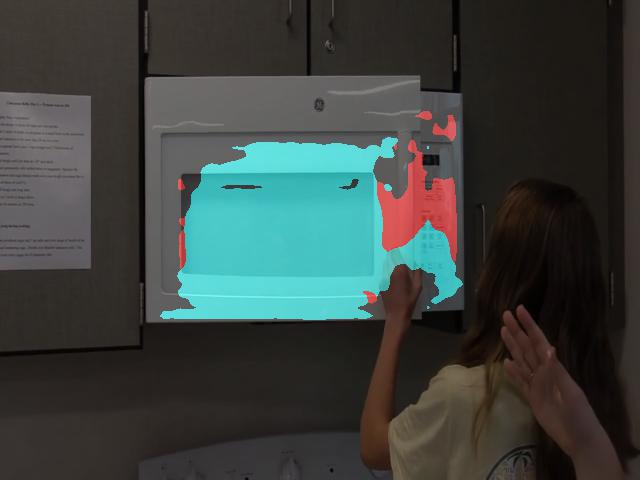
\includegraphics[width=0.15\textwidth]{example_wall/e01_no_normal/0_3_blend.jpg}}
    &\frame{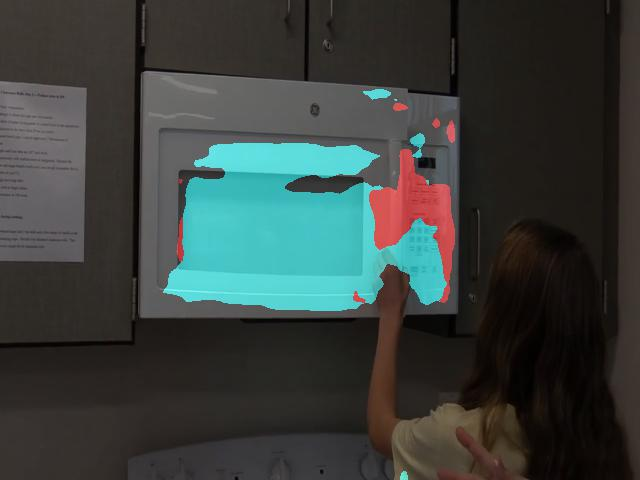
\includegraphics[width=0.15\textwidth]{example_wall/e01_no_normal/0_4_blend.jpg}} 
    &\frame{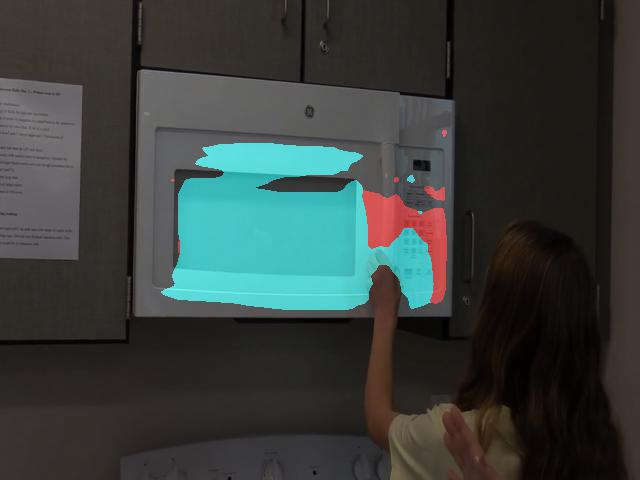
\includegraphics[width=0.15\textwidth]{example_wall/e01_no_normal/0_5_blend.jpg}}
    &\frame{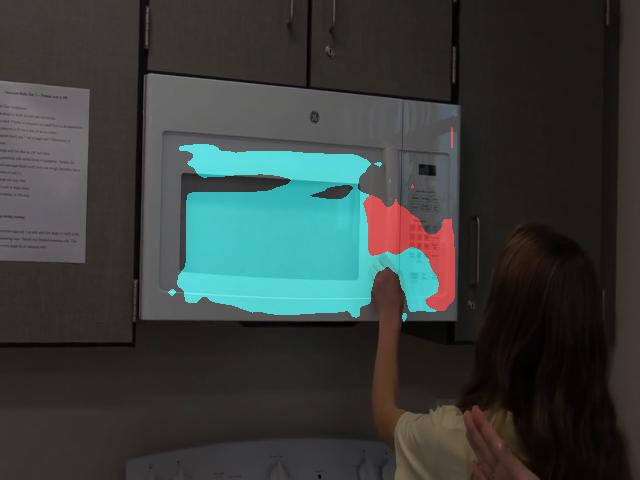
\includegraphics[width=0.15\textwidth]{example_wall/e01_no_normal/0_6_blend.jpg}} 
    &\frame{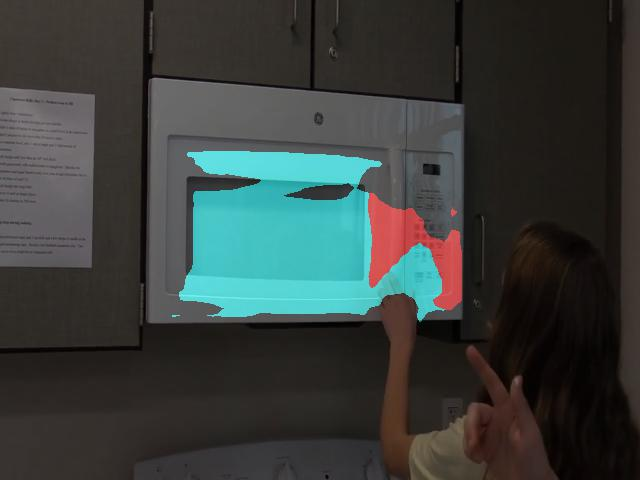
\includegraphics[width=0.15\textwidth]{example_wall/e01_no_normal/0_7_blend.jpg}} \\
    
    w/ normal
    &\frame{\includegraphics[width=0.15\textwidth]{example_wall/e01_ours/0_0_blend.jpg}} 
    &\frame{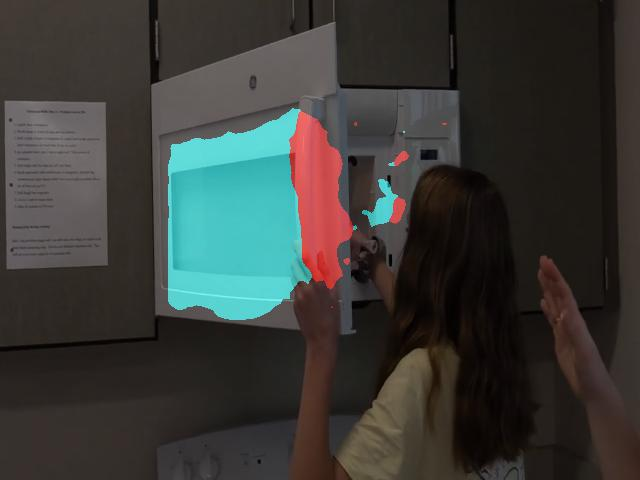
\includegraphics[width=0.15\textwidth]{example_wall/e01_ours/0_1_blend.jpg}}
    &\frame{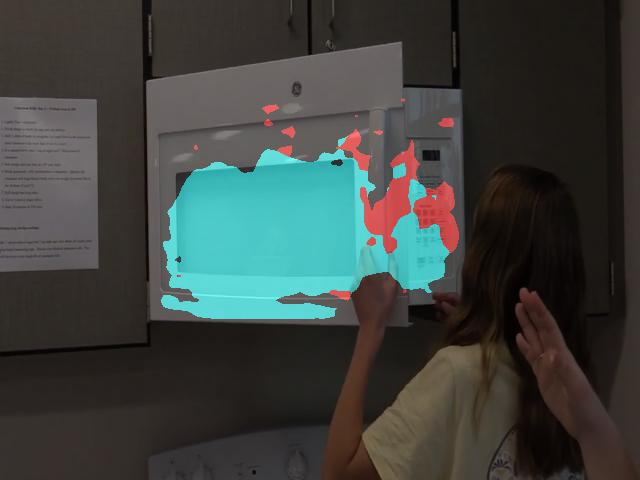
\includegraphics[width=0.15\textwidth]{example_wall/e01_ours/0_2_blend.jpg}} 
    &\frame{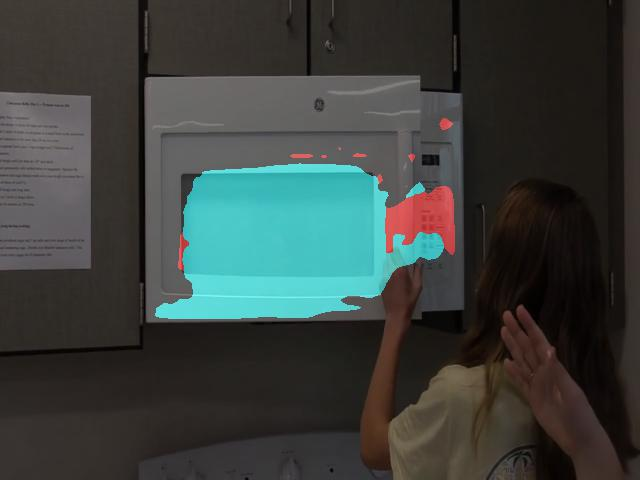
\includegraphics[width=0.15\textwidth]{example_wall/e01_ours/0_3_blend.jpg}}
    &\frame{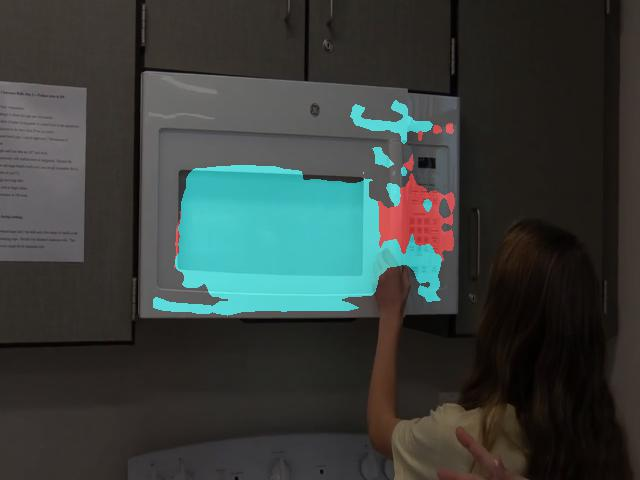
\includegraphics[width=0.15\textwidth]{example_wall/e01_ours/0_4_blend.jpg}} 
    &\frame{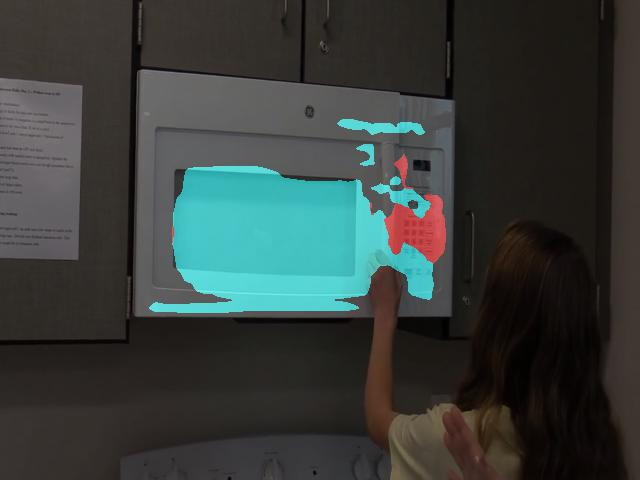
\includegraphics[width=0.15\textwidth]{example_wall/e01_ours/0_5_blend.jpg}}
    &\frame{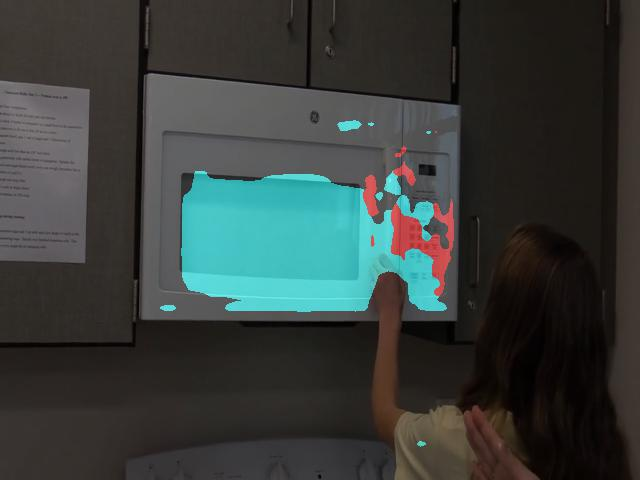
\includegraphics[width=0.15\textwidth]{example_wall/e01_ours/0_6_blend.jpg}} 
    &\frame{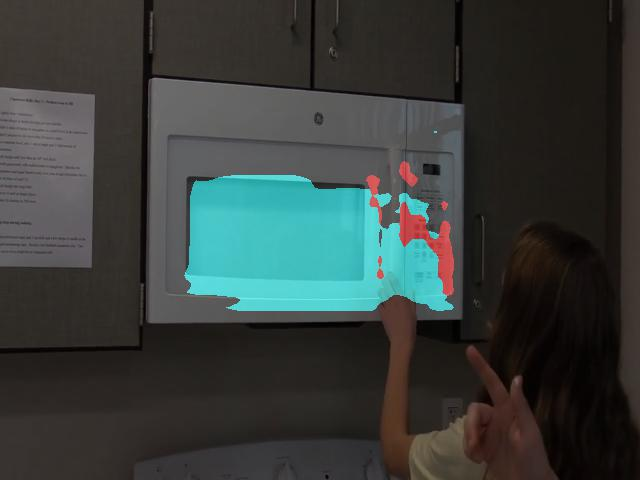
\includegraphics[width=0.15\textwidth]{example_wall/e01_ours/0_7_blend.jpg}} \\
    
    ~\cite{jabri2020walk} pretrained
    &\frame{\includegraphics[width=0.15\textwidth]{example_wall/e01_pretrained/0_0_blend.jpg}} 
    &\frame{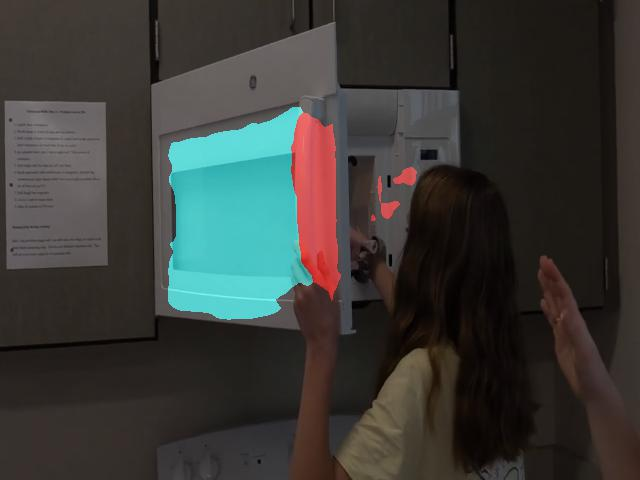
\includegraphics[width=0.15\textwidth]{example_wall/e01_pretrained/0_1_blend.jpg}}
    &\frame{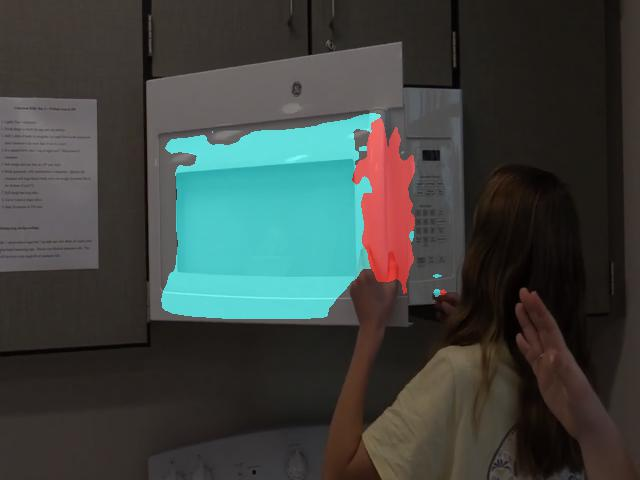
\includegraphics[width=0.15\textwidth]{example_wall/e01_pretrained/0_2_blend.jpg}} 
    &\frame{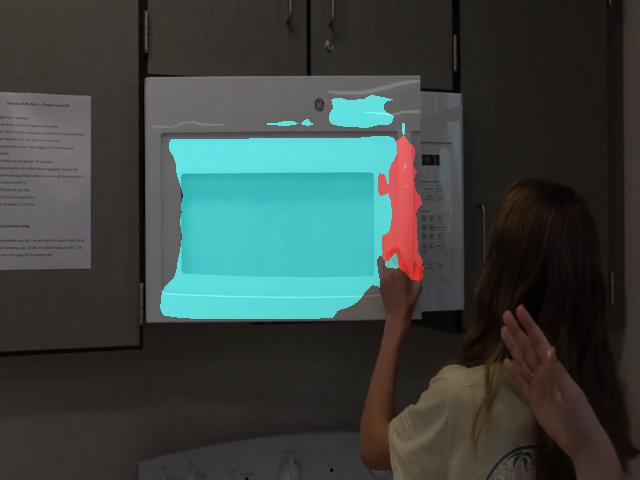
\includegraphics[width=0.15\textwidth]{example_wall/e01_pretrained/0_3_blend.jpg}}
    &\frame{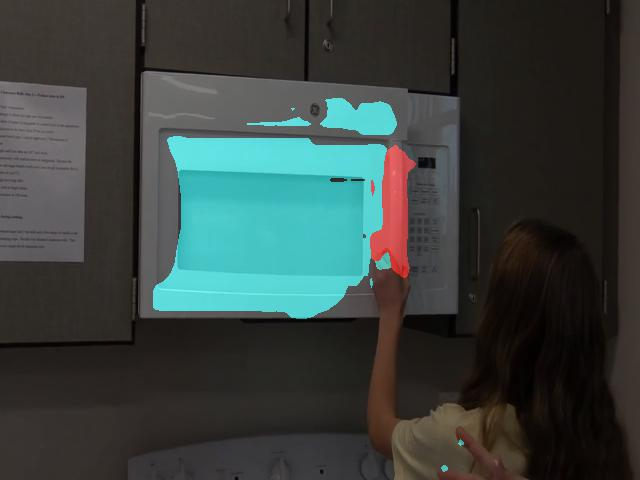
\includegraphics[width=0.15\textwidth]{example_wall/e01_pretrained/0_4_blend.jpg}} 
    &\frame{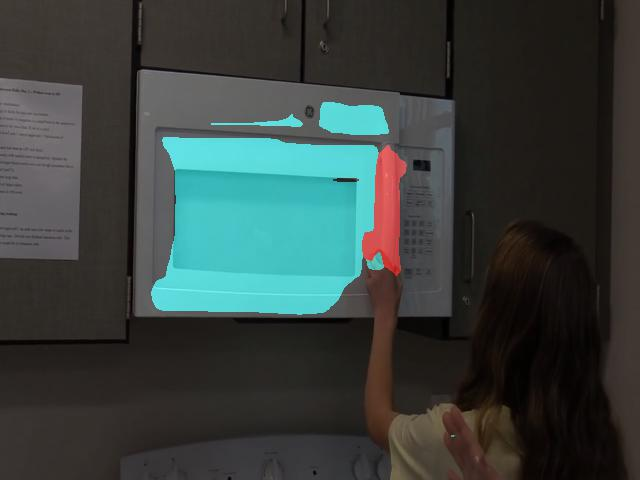
\includegraphics[width=0.15\textwidth]{example_wall/e01_pretrained/0_5_blend.jpg}}
    &\frame{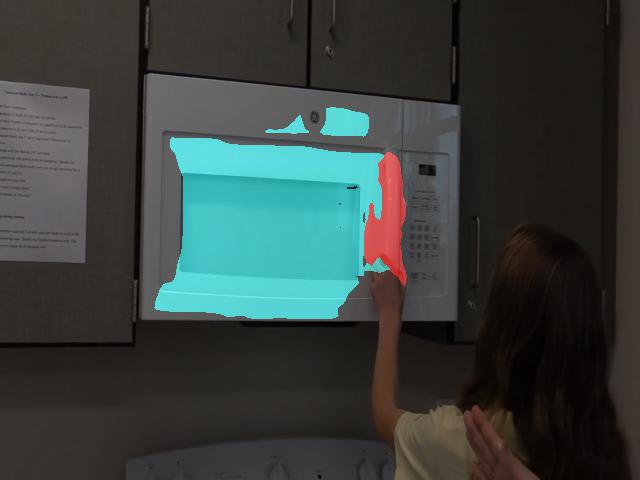
\includegraphics[width=0.15\textwidth]{example_wall/e01_pretrained/0_6_blend.jpg}} 
    &\frame{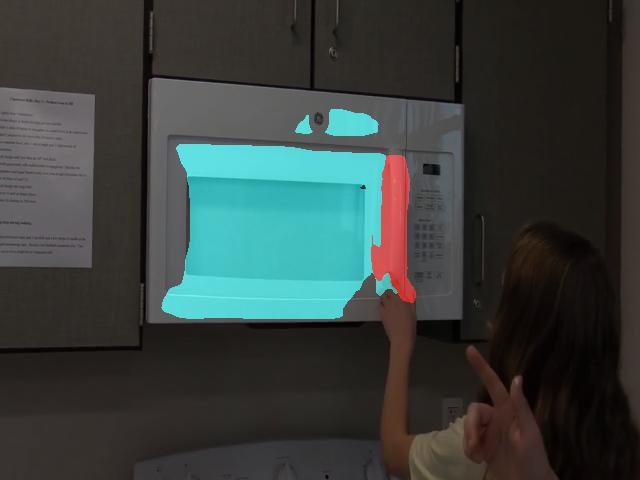
\includegraphics[width=0.15\textwidth]{example_wall/e01_pretrained/0_7_blend.jpg}} \\
    \bottomrule
    \end{tabular}
    }
    \vspace{-0.1in}
    
    \caption{Qualitative results on videos with dynamic scene of the label propagation task given an initial plane detection from PlaneRCNN model.}
    \label{fig:dynamic}
    \vspace{-0.2in}
\end{figure*}
%  dataset containing 2.5 million views in more than 1500 scans, annotated with 3D camera poses, surface reconstructions, and instance-level semantic segmentations.
We use ScanNet \cite{dai2017scannet} to train and evaluate our model for tracking 3D planes. ScanNet \cite{dai2017scannet} is an indoor RGB-D video dataset with surface reconstructions and instance segmentation annotations. The instance indices are consistent throughout the video frames which enables the evaluation for 3D object tracking. We downsample the image resolution from 1296 $\times$ 968 to 640 $\times$ 480 using bilinear interpolation. The instance masks are resized with the same ratio except that the nearest-neighbour interpolation is used to avoid introducing new instance indices. We use 10 scenes for training and 2 scenes for testing. Each scene contains 1000 to 5000 frames. See Figure \ref{fig:impair} and \ref{fig:mesh} for illustrations.


\subsection{Evaluation Metric}

We follow \cite{jabri2020walk} and two complementary criteria are employed to measure how our mask prediction $M$ fits the ground truth mask $G$. 

\par \noindent {\bf Region Similarity $\boldsymbol{J}$.} To measure the region-based segmentation similarity, the commonly used metric IoU (intersection-over-union, also known as the Jaccard index) is used. $J$ can be calculated as $J = \left| \frac{M \cap G}{M \cup G} \right|$.



\par \noindent {\bf Contour Accuracy $\boldsymbol{F}$.} Precision $P_c$ and recall $R_c$ can be calculated based on the contours extracted from $M$ and $G$. Then the F-measure $F$ can be calculated as $F = \frac{2P_cR_c}{P_c + R_c}$ to achieve a good trade-off between the two.

We follow \cite{jabri2020walk} to report mean (m) and recall (r) of the region similarity ($J$) and boundary alignment ($F$) \cite{perazzi2016benchmark}.


\begin{figure}[H]
  \centering
  \begin{subfigure}[b]{0.4\columnwidth}
    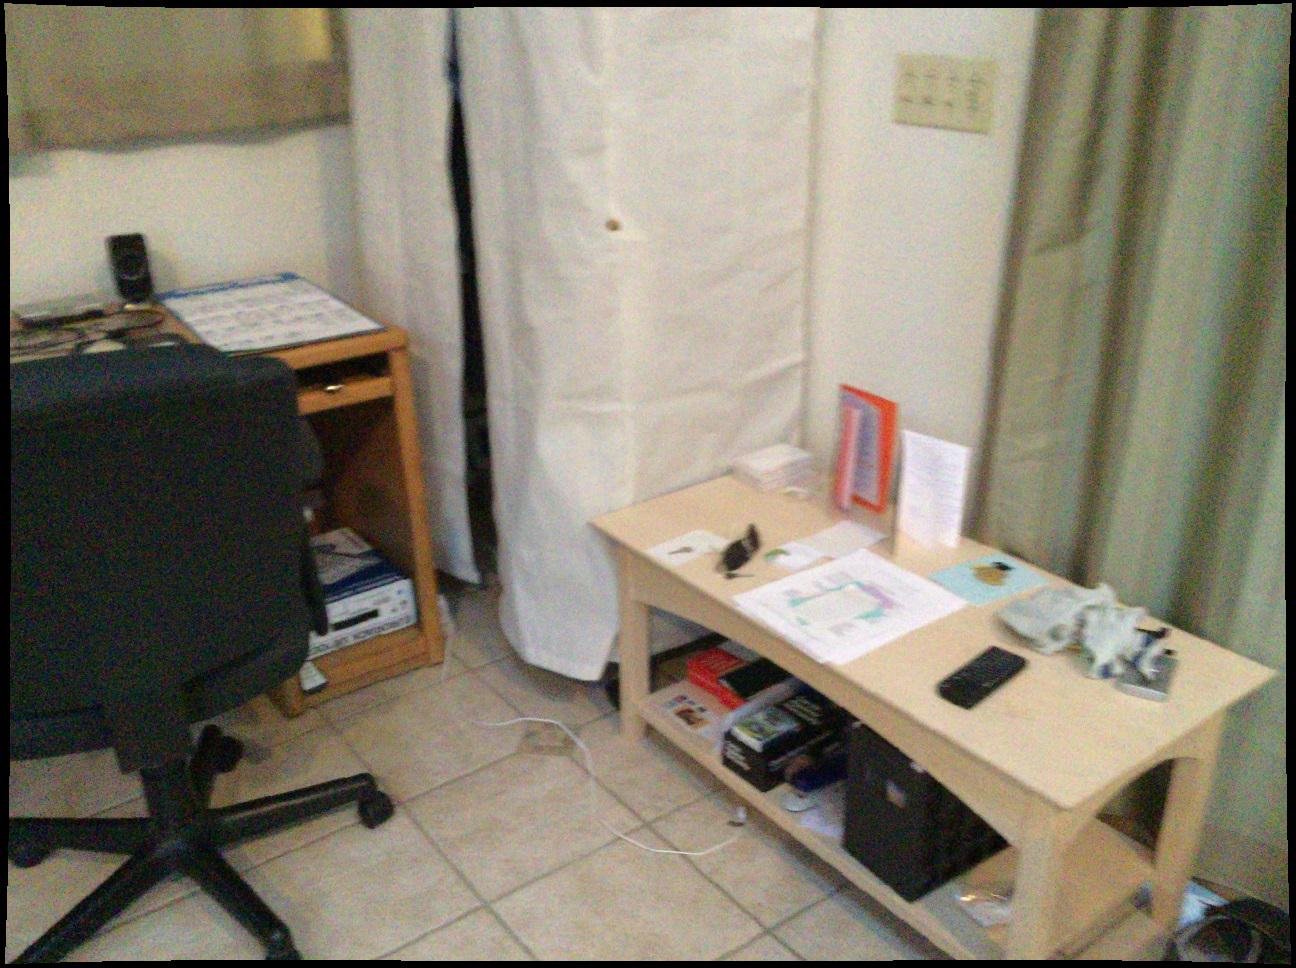
\includegraphics[width=\linewidth]{FinalReport/dataset_example/original.jpg}
    \caption{Scene Example}
  \end{subfigure}
  \begin{subfigure}[b]{0.4\columnwidth}
    
\includegraphics[width=\linewidth]{FinalReport/dataset_example/4.png}
    \caption{Instance Segmentation}
  \end{subfigure}
  \vspace{-0.1in}
  \caption{Image Mask Pair \cite{dai2017scannet}}
  \label{fig:impair}
      \vspace{-0.2in}
\end{figure}


% \vspace{-0.1in}
\begin{figure}[H]
  \centering
  \begin{subfigure}[b]{0.44\columnwidth}
    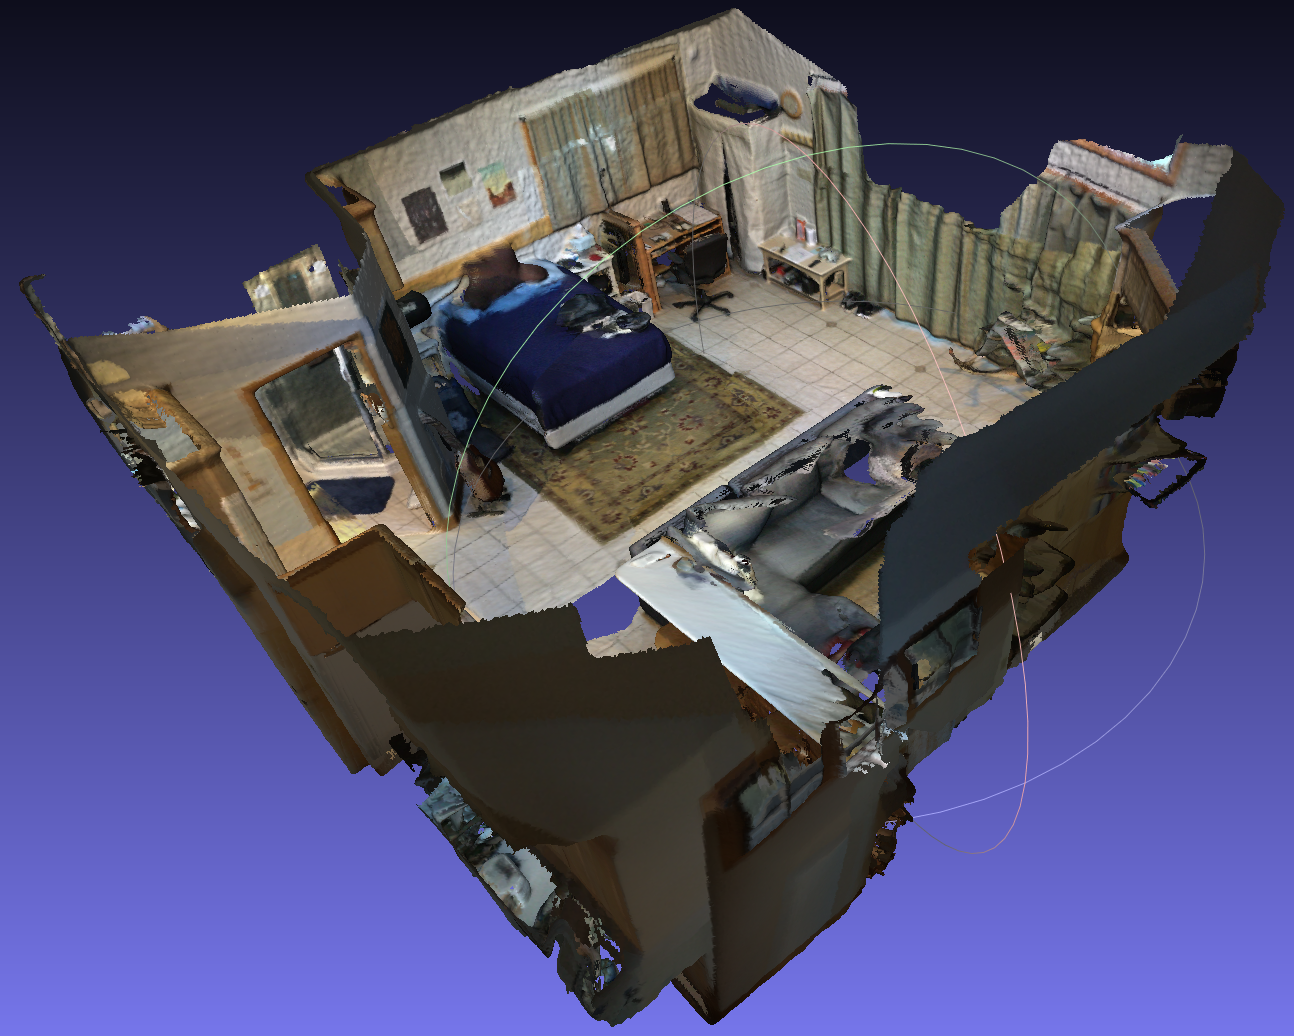
\includegraphics[width=\linewidth]{FinalReport/dataset_example/scene_mesh.png}
    \caption{Surface Reconstruction}

  \end{subfigure}
  \begin{subfigure}[b]{0.41\columnwidth}
    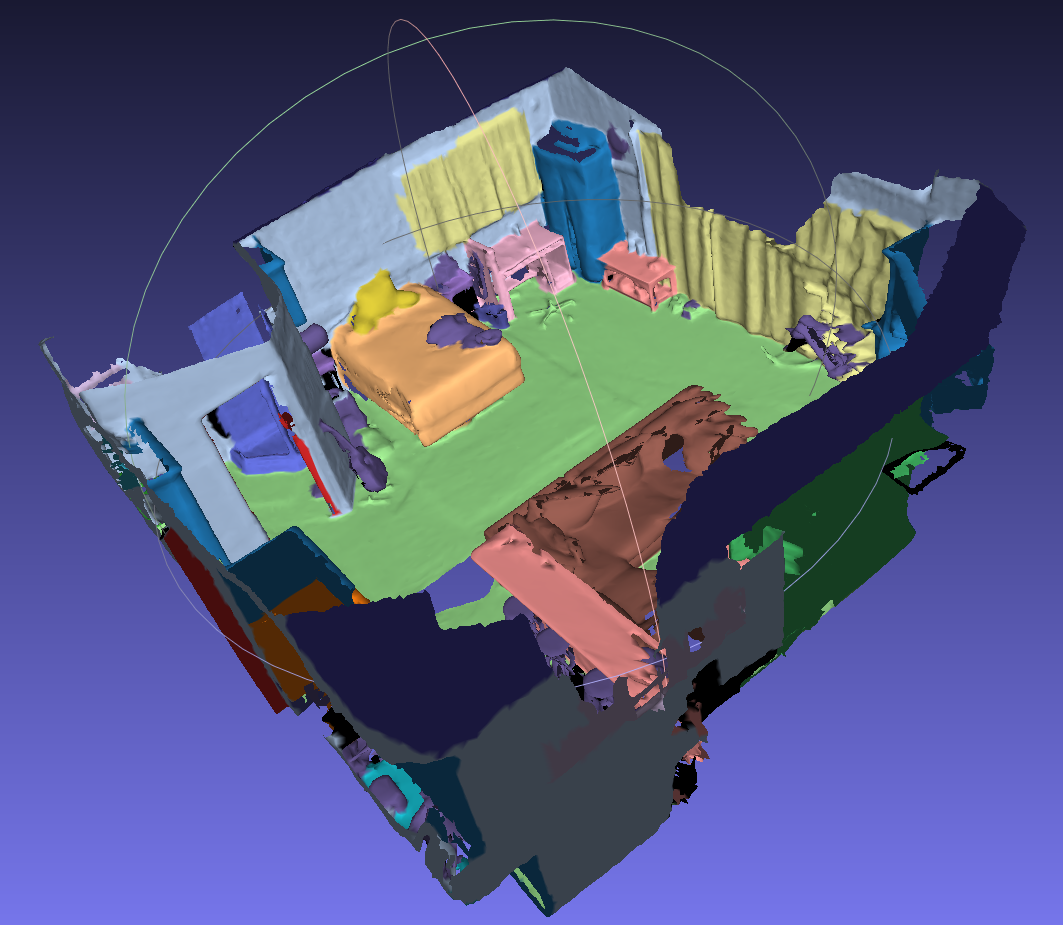
\includegraphics[width=\linewidth]{FinalReport/dataset_example/scene_label.png}
    \caption{Labeled Mesh}
  \end{subfigure}
    \vspace{-0.1in}
  \caption{Mesh Model \cite{dai2017scannet}}
      \vspace{-0.25in}
  \label{fig:mesh}
\end{figure}




\par \noindent {\bf Baselines.} We use two baseline models to compare with our proposed method. All models share the same network architecture. The first baseline is the pretrained model provided by \cite{jabri2020walk}, which only uses the self-supervised palindrome loss and is trained on the Kinetics400 \cite{carreira2017quo}. The second baseline is trained on a subset of the ScanNet scenes from scratch but without considering the surface normal constraints in the affinity matrix and the random-walk loss. Our model in contrast, is trained on the same subset of ScanNet from scratch and takes the normal difference into consideration as described in section \ref{sec:method}.

% \vspace{-0.2in}
\begin{figure}[H]
  \centering
  \begin{subfigure}[b]{0.85\columnwidth}
    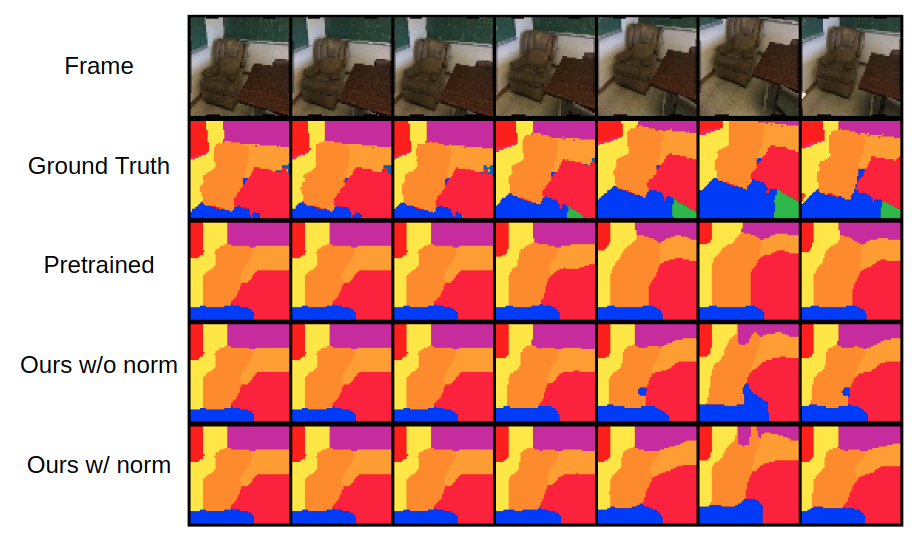
\includegraphics[width=\linewidth]{FinalReport/dataset_example/gt0030.png}
    \caption{Test scene A}
  \end{subfigure}
  \begin{subfigure}[b]{0.85\columnwidth}
    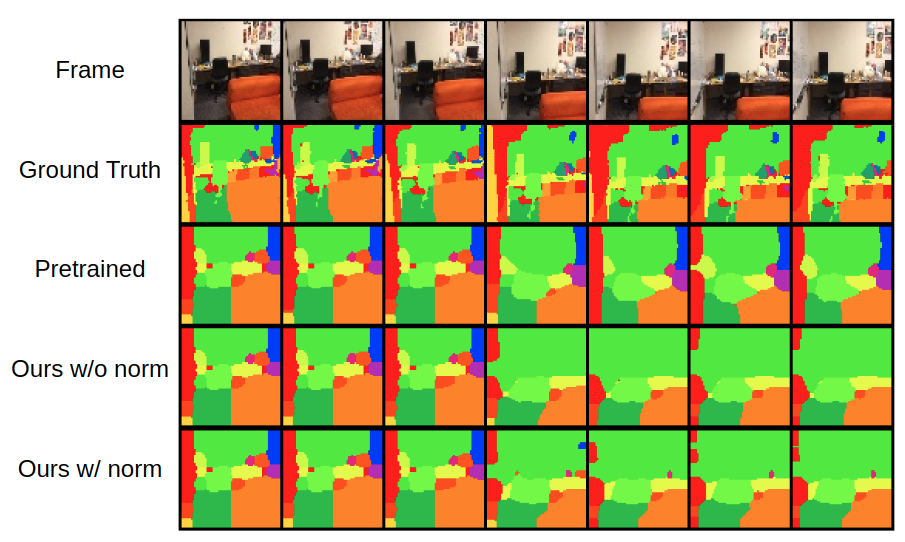
\includegraphics[width=\linewidth]{FinalReport/dataset_example/gt0040.png}
    \caption{Test scene B}
  \end{subfigure}
  \vspace{-0.1in}
  \caption{Test Scenes}
    \vspace{-0.3in}
  \label{fig:video_seg}
\end{figure}

\vspace{-0.05in}
% \titlespacing*{\subsection}{0pt}

\subsection{Qualitative Results}

We present some inference results from the two baseline models as well as our model, see Figure \ref{fig:video_seg}. The inference results are the instance segmentation masks of the scene, where the instance indices are consistent throughout the frames. We select two new scenes from the ScanNet dataset that are different from the training data in order to test the generalization ability of our model. 

% \TODO{interpretation here}
As shown in Figure \ref{fig:video_seg} a, our model with normal constraints can have denoising and smoothing effects on the plane detection (e.g. 5th column) compared with the model without normal constraints. However, it can also be subject to noises. As can be observed in Figure \ref{fig:video_seg} b, a small object with regional salient normal can induce noisy plane detection compared to the pretrained model (e.g. 7th column).

%\ref{fig:dynamic}
We also evaluate the methods on a dynamic scene, and the results are shown in Figure \ref{fig:dynamic}. All the three methods cannot predict the planes for the door and the handle perfectly, underlining the improvement space for our model on dynamic scenes.

\subsection{Quantitative Results}
Our quantitative results are listed in table \ref{table:quan}. Unsurprisingly, our model trained on the ScanNet \cite{dai2017scannet} outperforms the pretrained model \cite{jabri2020walk} on the test scenes because of the data distribution similarity. Our model with normal constraints slightly improves the model without normal constraints with limited training. This approach is promising if more training resources are available.

%%%% CONCLUSIONS
\section{Conclusions}
\label{sec:conclusions}
% \TODO{Please include the most important take-away message. This can be one paragraph about the reproducibility of the work, the strength/weakness of your method compared against baseline methods, and future work that can be done.}

While existing 3D objection detection methods are capable of handling difficult cases such as dynamic scenes, occlusion, and deformation, the prediction between frames are usually independent and thus is incapable of evaluating the temporal correspondence. We propose a new framework that builds on the video random-walk model \cite{jabri2020walk}, and integrates 3D information constraints into the affinity matrix and the loss function. Under our formulation, we observe slight improvement with the surface normal constraint with limited training. However, this approach can be subject to small and irregular planes and lead to noisy predictions. In the future work, this approach can be more thoroughly evaluated with more training, and other types of constraints can be applied such as plane texture.

\clearpage
{\small
\bibliographystyle{ieee_fullname}
\bibliography{egbib}
}

\end{document}
